\documentclass[oneside]{article}

\usepackage{natbib} % bibliography
\usepackage{blindtext} % dummy text
\usepackage{graphicx} % figures
\usepackage{color} % colored text
\usepackage{float} % forcing figure placement
\usepackage{enumerate} % for bullet point lists
\usepackage{setspace} % line spacing
\usepackage{booktabs} % horizontal rules in tables
\usepackage{amsmath} % text in equations
\usepackage{titlesec} % customization of titles
\usepackage{titling} % customizing the title section
\usepackage[breakable]{tcolorbox} % for text box
\usepackage[cache=false]{minted} % code boxes; FKM cache=false was
                                % necessary to work on my mac os X
% \usepackage{microtype} % slightly tweak font spacing for aestheticsgins
\usepackage[margin=1in]{geometry} % margins
\usepackage[breakable]{tcolorbox} % text box
\usepackage[sc]{mathpazo} % Palatino font
%\usepackage[T1]{fontenc} % use 8-bit encoding that has 256 glyphs
\usepackage[small,labelfont=bf,up,up]{caption} % custom captions under/above floats in tables or figures
\usepackage[hidelinks]{hyperref} % hyperlinks in the PDF

\usepackage{tikz}
\usepackage{bm}
\usetikzlibrary{bayesnet}

\usepackage{alltt}
\usepackage{lmodern}
\usepackage[T1]{fontenc}

\usepackage[shortlabels]{enumitem} % customized lists (shortlabels
                                % necessary to have i., ii., etc., in enumerate)
\setlist[itemize]{noitemsep} % make itemize lists more compact

\usepackage{abstract} % Allows abstract customization
\renewcommand{\abstractnamefont}{\normalfont\bfseries} % Set the "Abstract" text to bold
\renewcommand{\abstracttextfont}{\normalfont\small\itshape} % Set the abstract itself to small italic text

\usepackage{fancyhdr} % headers and footers
\pagestyle{fancy} % all pages have headers and footers
\fancyhead{} % blank out the default header
\fancyfoot{} % blank out the default footer
\fancyhead[C]{Authors et al. $\bullet$ August 2018 $\bullet$ bio{\color{red}R}$\chi$ve} % Custom header text
\fancyfoot[RO,LE]{\thepage} % Custom footer text

\let\oldtexttt\texttt% Store \texttt
\renewcommand{\texttt}[2][black]{\textcolor{#1}{\ttfamily #2}}% \texttt[<color>]{<stuff>}


\bibliographystyle{apalike}

\setlength\columnsep{20pt}

% lphy listing specification
\usepackage{listings}
\definecolor{bluevars}{rgb}{0.13,0.13,1}
\definecolor{redkeywords}{rgb}{0.5,0,0}
\definecolor{grayargs}{RGB}{169,169,169}

\lstnewenvironment{fslisting}
  {
    \lstset{
        language=FSharp,
        basicstyle=\ttfamily,
        breaklines=true,
        columns=fullflexible}
  }
  {
  }

\lstdefinelanguage{LPHY}{
  % more keywords specifies the distributions within lphy
  morekeywords={
    Yule,
    LogNormal,
    PhyloCTMC
  },
  keywordstyle=\color{redkeywords},
  sensitive=True
  }

\lstnewenvironment{lphylisting} {
  \lstset{
    mathescape=true,
    escapechar=*,
    language=LPHY,
    basicstyle=\ttfamily,
    breaklines=true,
    columns=fullflexible,
    % random variables
    emph={
      D,
      tree,
      lambda
    },
    emphstyle=\color{bluevars},
    % arguments to distributions
    emph={[2]
      file,
      sites,
      taxa,
      meanlog,
      sdlog,
      theta,
      L,
      Q,
      birthRate
    },
    emphstyle={[2]\color{grayargs}}
  }
}{}

%----------------------------------------------------------------------------------------
%	TITLE SECTION
%----------------------------------------------------------------------------------------

\pretitle{\begin{center}\Huge\bfseries} % title formatting
\posttitle{\end{center}} % title closing formatting
\title{Lingua Phylo: a probabilistic model specification language for
  reproducible phylogenetic analyses}
\author{\textsc{Alexei J. Drummond$^{1,2*}$}, \textsc{F\'{a}bio K. Mendes$^{1,2}$}\\%, \\ \textsc{Yet another author here$^{1*}$},
%  \textsc{Last author here$^{1*}$} \\
\small $^1$School of Biological Sciences, The University of Auckland\\
\small $^2$School of Computer Science, The University of Auckland\\
\small
\href{mailto:alexei@cs.auckland.ac.nz}{Corresponding author$^*$: alexei@cs.auckland.ac.nz}
%\href{mailto:someone@auckland.ac.nz}{another.email@auckland.ac.nz}
%\and % Uncomment if 2 authors are required, duplicate these 4 lines if more
%\textsc{Jane Smith}\thanks{Corresponding author} \\[1ex] % Second author's name
%\normalsize University of Utah \\ % Second author's institution
%\normalsize \href{mailto:jane@smith.com}{jane@smith.com} % Second author's email address
}
\date{\today} % Leave empty to omit a date
\renewcommand{\maketitlehookd}{%
\begin{abstract}
  Phylogenetic models have become increasingly complex and the data sets addressed larger and more rich.
  Yet there is no standard language to accurately specify the details of a phylogenetic model for the purposes of reproducibility or reuse.
  We present a new language to specify the details of a phylogenetic model that is both human and machine readable.
  We also report on the development of a graphical software package that can be used to construct and simulate data from
  models in this new language, as well as create natural language narratives that can form the basis of a description of the model for the method section of a manuscript.
  Finally we report on a command-line program that can be used to generate XML for the BEAST2 software package based
  on a model specified in this new language.
  These tools together should aid in the goal of reproducibility and reuse of probabilistic phylogenetic models.
\end{abstract}
\centering [Probabilistic models, Bayesian models, reproducibility]
}

%----------------------------------------------------------------------------------------

\doublespacing

\begin{document}

% Print the title
\maketitle

%----------------------------------------------------------------------------------------
%	ARTICLE CONTENTS
%----------------------------------------------------------------------------------------

\section{Introduction}

Transparency is a scientific ideal, and replicability and
reproducibility lie at the heart of the scientific endeavor
\citep{nas19,munafo17}.
Despite this being a non-contentious point, only recently have
systematic examinations of the literature begun to reveal that
reproducibility is largely overlooked in pratice.
Metaresearch efforts have uncovered the so-called ``reproducibility
crisis'' \citep{baker16} in many disciplines (but see
\citep{fanneli18}), among which the dimension of the problem varies.
In psychology, for example, a larger scale replication attempt was
successful in only 39\% of surveyed studies \citep{openscience15},
with numbers being less discouraging in other attempts (62\%;
\citep{camerer18}), and in other domains (e.g., economics, 61.1\%,
\citep{camerer16}; cancer biology, X\%, [citation]).

* In evolutionary biology we don't know very well yet, but some
initial papers show it also happens.

* Phylogenetics in particular is now highly computational, and the
intersection with computer science puts this area of evolutionary
biology in a special position to address reproducibility.

A new paradigm for scientific computing and data science has begun to
emerged in the last decade.
A recent example is the publication of the
first ``computationally reproducible article'' using eLife's
Reproducible Document Stack which blends features of a traditional
manuscript with live code, data and interactive figures.

Although standard tools for statistical phylogenetics provide a degree
of reproducibility and reusability through popular open-source
software and computer-readable data file formats, there is still much
to do.
The ability to construct and accurately communicate
probabilistic models in phylogenetics is frustratingly
underdeveloped.
There is low interoperability between different
inference packages (e.g. BEAST1, BEAST2, MrBayes, RevBayes), and the
file formats that these software use have low readability for
researchers.

In this paper we describe two related projects, LinguaPhylo (LPhy for
short) and LPhyBEAST.

\section{LinguaPhylo}

\subsection{Why do we need a new language?}


\subsubsection{Enhance communication and hide unnecessary details}

A concise formal language to describe only the data and model would enable easy yet precise communication about modelling and inference intentions, without the need to understand all the implementation details of a particular software package. This is akin to the concept of encapsulation in object-oriented programming. We want to avoid exposing users to unnecessary complexity of implementation details.
Current input files for popular Bayesian inference software are replete with unnecessary implementation details.
For example the BEAST2 input file format exposes the user to a wide array of details beyond the statistical model and data:
\begin{itemize}
\item The XML language
\item A mapping from XML to Java classes in the BEAST2 source code
\item The Java class names defined in the BEAST2 source code
\item A model structure dictated by the internal BEASTObject hierarchy in BEAST2 source code
\item Operator schedules, weights {\it et cetera}
\item Details of the output loggers
\end{itemize}

\subsubsection{Enable a richer modelling universe that is more expressive}

By focusing on a modular high-level language acting on a small number of fundamental data types, this new modelling language naturally lends itself to greater expressivity.

LinguaPhylo is a model specification language to concisely and
precisely define probabilistic phylogenetic models.
The aim is to work
towards a common language for probabilistic models of phylogenetic
evolution.
This language should be readable by both humans and
computers.
Here is an example:

\begin{tcolorbox}[breakable, width=\textwidth, colback=gray!10, boxrule=0pt,
  title=Box 1: A simple molecular phylogenetic model, fonttitle=\bfseries]
  \begin{minipage}[t]{0.60\textwidth}
  (a) Modeling language
\\
    {\singlespacing
\begin{alltt}
model \{
  \textcolor{green}{\(\lambda\)} ~ \textcolor{blue}{LogNormal}(\textcolor{gray}{meanlog=}\textcolor{magenta}{3.0}, \textcolor{gray}{sdlog=}\textcolor{magenta}{1.0});
  \textcolor{green}{\(\psi\)} ~ \textcolor{blue}{Yule}(\textcolor{gray}{lambda=}\textcolor{green}{\(\lambda\)}, \textcolor{gray}{n=}\textcolor{magenta}{16});
  \textcolor{green}{D} ~ \textcolor{blue}{PhyloCTMC}(\textcolor{gray}{L=}\textcolor{magenta}{200}, \textcolor{gray}{Q=}\textcolor{magenta!80!black}{jukesCantor}(), \textcolor{gray}{tree=}\textcolor{green}{\(\psi\)});
\}
\end{alltt}
}
(c) Posterior

$$P(\psi, \lambda | D) \propto P(D | \psi) P(\psi | \lambda) P(\lambda) $$

  \end{minipage}%
\begin{minipage}[t]{0.40\textwidth}
(b) Graphical model
\\\\
\centering
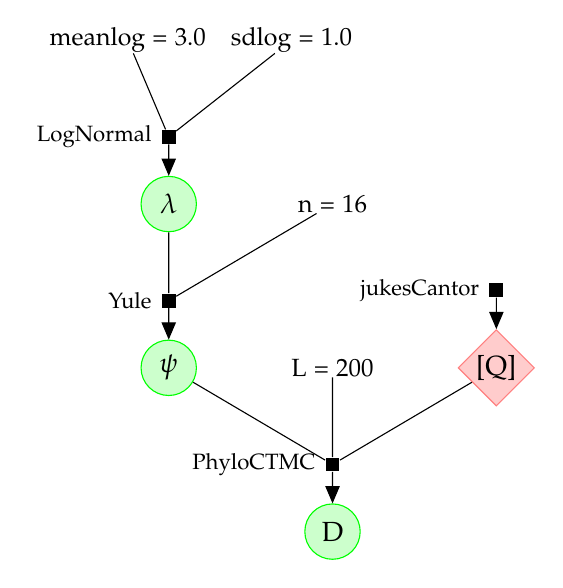
\begin{tikzpicture}[scale=0.52,
dstyle/.style={draw=blue!50,fill=blue!20},
vstyle/.style={draw=green,fill=green!20},
cstyle/.style={font=\small},
detstyle/.style={draw=red!50,fill=red!20}
]
\node[const, cstyle] at (1.0, -0.0) (602717583) {meanlog = 3.0};
\node[const, cstyle] at (5.0, -0.0) (897996787) {sdlog = 1.0};
\node[latent, vstyle] at (2.0, -4.0) (lambda) {$\lambda$};
\node[const, cstyle] at (6.0, -4.0) (2011155364) {n = 16};
\node[latent, vstyle] at (2.0, -8.0) (psi) {$\psi$};
\node[const, cstyle] at (6.0, -8.0) (1992433642) {L = 200};
\node[det, detstyle] at (10.0, -8.0) (258223775) {[Q]};
\node[latent, vstyle] at (6.0, -12.0) (D) {D};
\factor[above=of lambda] {LogNormallambda} {left:LogNormal} {} {} ; %
\factoredge {602717583, 897996787} {LogNormallambda} {lambda}; %
\factor[above=of psi] {Yulepsi} {left:Yule} {} {} ; %
\factoredge {lambda, 2011155364} {Yulepsi} {psi}; %
\factor[above=of 258223775] {jukesCantor258223775} {left:jukesCantor} {} {} ; %
\factoredge {} {jukesCantor258223775} {258223775}; %
\factor[above=of D] {PhyloCTMCD} {left:PhyloCTMC} {} {} ; %
\factoredge {1992433642, 258223775, psi} {PhyloCTMCD} {D}; %
\end{tikzpicture}
%   \begin{tikzpicture}[scale=0.5,
%dstyle/.style={draw=blue!50,fill=blue!20},
%vstyle/.style={draw=green,fill=green!20},
%detstyle/.style={draw=red!50,fill=red!20}
%]
%\node[latent, vstyle] at (0.0, -2.0) (lambda) {$\lambda$};
%\node[latent, vstyle] at (0.0, -6.0) (psi) {$\psi$};
%\node[latent, vstyle] at (0.0, -10.0) (D) {D};
%\factor[above=of lambda] {LogNormallambda} {left:LogNormal} {} {} ; %
%\factoredge {} {LogNormallambda} {lambda}; %
%\factor[above=of psi] {Yulepsi} {left:Yule} {} {} ; %
%\factoredge {lambda} {Yulepsi} {psi}; %
%\factor[above=of D] {PhyloCTMCD} {left:PhyloCTMC} {} {} ; %
%\factoredge {psi} {PhyloCTMCD} {D}; %
%\end{tikzpicture}
  \end{minipage}


  % {\singlespacing
  % \begin{minted}{Stan}
  % model {
  % lambda ~ LogNormal(meanlog=3.0, sdlog=1.0);
  % tree ~ Yule(lambda=lambda, n=16);
  % D ~ PhyloCTMC(L=200, Q=jukesCantor(), tree=tree);
  % }
  % \end{minted}
  % }

\end{tcolorbox}
Each of the lines in this model specification expresses how a random
variable (to the left of the tilde) is generated by a generative
distribution to the right.

The first line creates a random variable (\texttt{lambda}), that is
log-normally distributed.
The second line creates a tree (\texttt{tree}) with 16 taxa from the
Yule process with a lineage birth rate equal to \texttt{lambda}.
The third line produces a multiple sequence alignment (\texttt{D})
with a length of 200, by simulating a Jukes Cantor model of sequence
evolution down the branches of  \texttt{tree}.
As you can see, each of the random variables depends on the previous,
so this is a hierarchical model that ultimately defines a probability
distribution over sequence alignments of size $16 \times 200$.

To construct an analysis of a data set with this model we add a data block:

{\singlespacing
\begin{minted}{Stan}
data {
  D = nexus(file="examples/primate.nex");
  L = D.nchar();
  taxa = D.taxa();
}
model {
  lambda ~ LogNormal(meanlog=3.0, sdlog=1.0);
  tree ~ Yule(lambda=lambda, taxa=taxa);
  D ~ PhyloCTMC(L=L, Q=jukesCantor(), tree=tree);
}
\end{minted}
}

These two blocks of statements contain all the information needed to define
a Bayesian phylogenetic analysis of a multiple sequence alignment.
The data block may contain literals, and deterministic values, including those read in from a file, but not random variables or generative distributions.
The model block contains all random variables, generative distributions and boundary conditions that define the model.
If a value in the data block has the same name as a random variable in the model block, then that signifies that the data block value is an observation of the random variable with the same name.


So by assigning the alignment in file
``primate.nex'' to the name D in the data block we are saying that the random variable in the model named D has
been observed, and we will infer all the other random variables
(tree and lambda in this example) in the model from that observed sequence alignment.

\subsection{Language features}

LinguaPhylo has two main components: Values (which can be either constant or random variables, and either objects or primitives) and Generators (which can be either generative distributions, deterministic functions or method calls).

\subsection{Values}

\subsection{Primitive constants}

The simplest type of value in LinguaPhylo is a primitive constant such in the following example. The first line defines a constant named `a' with a value of `2.0'. There is no explicit statement of the type, which is simply inferred to be a Double because the literal string `2.0' has a fractional component. The second constant `b' here is a constant of type Integer because it has no decimal point or fractional component. The third constant is of primitive type Boolean, inferred by the keyword `true'. the last constant is of type String because of the double quotes surrounding the literal value.

{\singlespacing
\begin{minted}{Stan}
  a = 2.0;
  b = 2;
  c = true;
  d = "lphy";
\end{minted}
}

\subsection{Arrays}

The notion of primitives can be extended to arrays and to declare a constant array you can enclose comma-delimited literals in square brackets as shown below. For sequences of consecutive integers a more compact notation can be employed using the `:' to define a range. In the example below a and b represent the same constant array containing the consecutive integers from 1 to 10 inclusive.

\begin{minted}{Stan}
  a = [1,2,3,4,5,6,7,8,9,10];
  b = 1:10;
\end{minted}

\subsection{Generative distributions}

A generative distribution generates a named random variable which has a value that is either an object or a primitive. Some generative distributions have parameters which have argument labels

{\singlespacing
\begin{minted}{Stan}
  lambda ~ LogNormal(meanlog=3.0, sdlog=1.0);
\end{minted}
}

\subsection{Deterministic functions}

A deterministic function generates either an object or a primitive value that is a deterministic function of its arguments. If the function has a single argument then no argument label is needed, otherwise arguments are labelled in the same way as for generative distributions. In the code below the function named hky takes two parameters with argument labels `kappa' and `freq' and deterministically produces an instantaneous rate matrix using those values.

{\singlespacing
\begin{minted}{Stan}
  Q = hky(kappa=2.0, freq=[0.2, 0.25, 0.4, 0.15]);
\end{minted}
}

\subsection{Vectorization}

LinguaPhylo has built-in vectorization so that any distribution or function can be called with a vectorized form of its arguments to produce multiple values from the generator

\section{Tree generative distributions}

There are many statistical programming languages such as Stan
\cite{carpenter2017stan}, JAGS \cite{plummer2003jags} and BUGS \cite{lunn2009bugs, gilks1994language} that provide the possibility
of succinctly describing statistical models. The unique model feature of
phylogenetic analysis is the phylogenetic tree.
This is a complex high-dimensional object, part discrete, part
continuous.
There is no bijection between tree space and Euclidean space, so it
can not be treated with standard statistical distributions.
As a result specialist software is needed to perform inference \cite{hohna2016revbayes,bouckaert2019beastanalysis}.

The aim of LPhy is describe the standard phylogenetic tree
distributions succinctly and precisely, while leaving out trivial algorithmic details related to the method
of inference and the particular software employed to do the inference.

\subsection{Coalescent generative distributions for time trees}

LPhy has describes a family of coalescent generative distributions
that produce TimeTrees.

The simplest model in this package is the one parameter model
constant-population size coalescent.
The generation-time-scaled population size parameter (theta) parameter determines at
what rate, per unit time, a pair of lineages coalesce, backwards in time.

\subsubsection{Constant population size coalescent model}

In its simplest form (Kingman; 1981) the coalescent model produces a
tree on a fixed number of leaves based on a population size parameter (theta):

\begin{minted}{Stan}
g ~ Coalescent(theta=0.1, n=16);
\end{minted}

It is also possible to give explicit taxa labels to the generative
distribution:

\begin{minted}{Stan}
g ~ Coalescent(theta=0.1, taxa=["a", "b", "c", "d"]);
\end{minted}

It is also possible to handle serially-sampled (time-stamped) data by
adding ages.
There are two ways to do that:

Ages without taxa names:

\begin{minted}{Stan}
g ~ Coalescent(theta=0.1, ages=[0.0, 0.1, 0.2, 0.3]);
\end{minted}

Ages and taxa names:

\begin{minted}{Stan}
taxaAges = taxaAges(taxa=["a", "b", "c", "d"], ages=[0.0, 0.1, 0.2,
0.3]);
g ~ Coalescent(theta=0.1, taxaAges=taxaAges);
\end{minted}

\subsubsection{Classic skyline coalescent model}

A highly parametric version of the coalescent is also possible, where
a series of theta values are provided, one for each group of consecutive coalescent intervals.
If the groupSizes are specified then each coalescent interval is given its
own population size.
The following code would generate a tree of five taxa, since there are four theta values provided:

\begin{minted}{Stan}
g ~ SkylineCoalescent(theta=[0.1, 0.2, 0.3, 0.4]);
\end{minted}

The theta values are indexed from the present into the past.
So the first coalescent interval (starting from the leaves)
would be generated assuming a population size parameter of 0.1, while
the last coalescent interval (culimating at the root of the tree)
would be generated from a population size parameter of 0.4.

It is also possible to add taxa and/or taxa age information:

\begin{minted}{Stan}
taxaAges = taxaAges(taxa=["a", "b", "c", "d"], ages=[0.0, 0.1, 0.2, 0.3]);
g ~ SkylineCoalescent(theta=[0.1, 0.2, 0.3], taxaAges=taxaAges);
\end{minted}

This will produce a serial coalescent tree with three distinct epochs
of population size on four taxa with distinct ages.

\subsubsection{Generalized skyline coalescent model}

The following generative distribution call will produce a tree of size
n=11 taxa, since 4+3+2+1=10= coalescent intervals.
The first four intervals will all have theta=0.1, the next three will
have theta=0.2, the next two will have theta=0.3, and the last
coalescent interval will have theta=0.4:

\begin{minted}{Stan}
g ~ SkylineCoalescent(theta=[0.1, 0.2, 0.3, 0.4], groupSizes=[4,3,2,1]);
\end{minted}

\subsubsection{Structured coalescent}

A structured coalescent process takes a migration matrix (M) with
population sizes of each deme on the diagonal:
For K demes, theta is an K-tuple and the dimension of m is $K^2 -
K$. $n$ is a tuple of sample sizes, one dimension for each deme:

\begin{minted}{Stan}
M = migrationMatrix(theta=[0.1, 0.1], m=[1.0, 1.0]);
g ~ StructuredCoalescent(M=M, n=[15, 15]);
\end{minted}

\subsubsection{Multispecies coalescent}

This model allows for gene tree-species tree discordance, and is a
hierarchical model of phylogeny.
A simple multispecies coalescent model has one distribution define a
species tree, and a second distribution define a gene tree based on
the species tree:

\begin{minted}{Stan}
S ~ Yule(lambda=5, n=4);
theta = [0.1, 0.1, 0.1, 0.1, 0.1, 0.1, 0.1];
g ~ MultispeciesCoalescent(theta=theta, n=[2, 2, 2, 2], S=S);
\end{minted}

Each branch in the species tree has its own theta value.
The $n$ value describes how many individuals are represented in
the gene tree for each species.
It is a tuple of integers with length equal to the number of species
in the species tree.

\subsection{Birth-death process generative distributions of trees}

The other main family of tree distributions is the birth-death-sampling generative distributions.

The simplest model in this family is the one parameter model Yule model \cite{yule1925ii}.
The birth rate (lambda) parameter determines at what rate, per unit time, each lineage bifurcates to produce two daughter lineages.
This describes a pure birth process, so that the number of lineages grows monotonically forward in time.

\subsubsection{Yule model}

In its simplest form the Yule model has a stopping criterion based on the final number of leaves in the tree.
The following code will generate a random Yule tree with 16 leaves:

\begin{minted}{Stan}
tree ~ Yule(lambda=1.0, n=16);
\end{minted}

It is also possible to give explicit taxa labels to the generative distribution:

\begin{minted}{Stan}
taxa = 1:16;
tree ~ Yule(lambda=1.0, taxa=taxa);
\end{minted}

or

\begin{minted}{Stan}
taxa = ["A", "B", "C", "D"];
tree ~ Yule(lambda=1.0, taxa=taxa);
\end{minted}

\subsubsection{Calibrated Yule model}

It is also possible the generate a Yule tree with a given rootAge:

\begin{minted}{Stan}
tree ~ Yule(lambda=1.0, n=16, rootAge=10);
\end{minted}

This is useful if you want to produce a calibrated analysis where there is a separate prior on the root age of the tree:

\begin{minted}{Stan}
rootAge ~ LogNormal(meanlog=2.0, sdlog=1.0);
tree ~ Yule(lambda=1.0, n=16, rootAge=rootAge);
\end{minted}

\subsubsection{Birth-death model}

The birth-death tree process is a generalisation of the Yule model. A second rate of extinction (mu) is added alongside
the rate of speciation (lambda). Running forward in time it is possible for the number of lineages to both grow and
shrink, and indeed for the tree process to go completely extinct.

\subsubsection{Calibrated Birth-Death process}

A calibrated birth-death process can be describe like so:

\begin{minted}{Stan}
tree ~ BirthDeath(lambda=2.0, mu=1.0, n=16, rootAge=10);
\end{minted}

It is important to realise that the resulting tree will contain only the extant lineages. All extinct lineages will be
suppressed. As with the Yule model it is possible to directly specify the taxa names:

\begin{minted}{Stan}
taxa = ["A", "B", "C", "D"];
tree ~ BirthDeath(lambda=2.0, mu=1.0, taxa=taxa, rootAge=10);
\end{minted}

\subsubsection{Full birth-death process}

It is possible to generate a full birth-death tree that includes also extinct lineages using the following generative
distribution:

\begin{minted}{Stan}
tree ~ FullBirthDeath(lambda=2.0, mu=1.0, rootAge=10);
\end{minted}

Note that unlike the BirthDeath generative distribution, this process will generate a tree with a random number of
leaf nodes, both in terms of extinct and extant lineages. The only conditioning is on the root age.

\subsubsection{Birth-death-sampling process}

A birth-death-sampling process adds a third parameter (rho) the probability of sampling each extant lineage. Again,
only extant lineages are leaves in the resulting tree and extinct lineages are suppressed:

\begin{minted}{Stan}
T ~ BirthDeathSampling(lambda=2.0, mu=1.0, rho=0.5, rootAge=3);
\end{minted}

An alternative parameterization allows specification of the diversification and turnover rates:

\begin{minted}{Stan}
T ~ BirthDeathSampling(diversification=1.0, turnover=0.5, rho=0.5, rootAge=3);
\end{minted}

Again it is important to note that the number of tips of the tree is a random variable, and is not conditioned on,
unlike for the BirthDeath generative distribution above.

\subsubsection{Birth-death-serial-sampling process}

A birth-death-serial-sampling \cite{stadler2013dating} process adds a fourth parameter (psi), the rate of sampling each lineage per unit time.
Now leaves of the tree can either be extinct (psi-sampled) or extant (rho-sampled).

\begin{minted}{Stan}
ages = [0.0,1.0,2.0,3.0,4.0];
tree ~ BirthDeathSerialSampling(lambda=1, mu=0.5, rho=0.1, psi=1, rootAge=5, ages=ages);
\end{minted}

In this case the number of leaves in the tree, and their ages are conditioned on, so are not random variables.

\section{Models of evolutionary rates and sequence evolution}

Another key distribution necessary to perform phylogenetic inference
is the phylogenetic continuous-time Markov process and its inference
equivalent the phylogenetic likelihood \cite{felsenstein1981}.

In its simplest form the PhyloCTMC generative
distribution takes an instantaneous transition matrix (Q), a number of sites (L) and a tree:

\begin{minted}{Stan}
tree = newick(tree="((A:0.1,B:0.1):0.2,(C:0.15,D:0.15):0.15);");
D ~ PhyloCTMC(tree=tree, Q=jukesCantor(), L=100);
\end{minted}

\subsection{ Molecular clock}

If the tree is not in units of substitutions per site, then it is possible to include a molecular clock rate
to scale the branches of the tree from time to substitutions per site. This example will give the same
result as the previous example, but the tree is now in units of time, so the mutation rate (mu) in units of
substitutions per site per unit time is given.

\begin{minted}{Stan}
tree = newick(tree="((A:10,B:10):20,(C:15,D:15):15);");
D ~ PhyloCTMC(tree=tree, Q=jukesCantor(), L=100, mu=0.01);
\end{minted}

\subsection{ Nucleotide substitution models}

There are a number of built in functions to construct standard nucleotide rate matrices. Some examples:

\begin{minted}{Stan}
jc = jukesCantor();
hky = hky(kappa=2.0, freq=[0.2, 0.25, 0.3, 0.25]);
gtr = gtr(rates=[0.1, 0.25, 0.15, 0.15, 0.25, 0.1], freq=[0.2, 0.25, 0.3, 0.25]);
\end{minted}

The Dirichlet prior is a natural prior for relative rates and frequencies, so a full model for GTR could
look like this:

\begin{minted}{Stan}
pi ~ Dirichlet(conc=[3.0,3.0,3.0,3.0]); // dirichlet prior on base frequencies
R ~ Dirichlet(conc=[1.0, 2.0, 1.0, 1.0, 2.0, 1.0]); // dirichlet prior on relative rates
Q = gtr(freq=pi, rates=R); // construct the GTR instantaneous rate matrix
\end{minted}

\subsection{ Rate heterogeneity across sites}

The PhyloCTMC generative distribution takes a parameter siteRates to describe rates across sites.
For inference, a common model is the discretized Gamma distribution of site rate heterogeneity (Yang, 1994).

To match this model for simulation in LPHY do the following:

\begin{minted}{Stan}
tree = newick(tree="((A:0.1,B:0.1):0.2,(C:0.15,D:0.15):0.15);");
siteRates ~ G(shape=0.5, ncat=4, reps=100); // generate 100 site rates from a discretized Gamma
D ~ PhyloCTMC(tree=tree, Q=jukesCantor(), siteRates=siteRates);
\end{minted}

\subsection{  Relaxed clock models (rate heterogeneity across branches) }

The PhyloCTMC generative distribution can also take an optional parameter branchRates to describe the
rates across branches:

\begin{minted}{Stan}
tree = newick(tree="((A:0.1,B:0.1):0.2,(C:0.15,D:0.15):0.15);");
branchRates = [0.5, 2.0, 1.0, 1.0, 2.0, 0.5];
D ~ PhyloCTMC(L=100, Q=jukesCantor(), tree=tree, branchRates=branchRates);
\end{minted}

\section{LinguaPhylo Studio}

Along with the language definition, we also provide software to
specify and visualise models as well as simulate data from models
defined in LPhy.

This software will also provide the ability for models specified in
the LPhy language to be applied to data using standard inference tools
such as MrBayes, RevBayes, BEAST1 and BEAST2
\cite{bouckaert2014beastanalysis,DrummondBouckaert2015,bouckaert2019beastanalysis}.
This will require software that can convert an LPhy specification into
an input file that these inference engines understand.
The first such software converter is LPhyBEAST described below.

\section{LPhyBEAST}

LPhyBEAST is a command-line program that takes an LPhy model
specification, and some data and produces a BEAST 2 XML input file.
It is therefore an alternative way to succinctly express and
communicate BEAST analyses.

%\bibliographystyle{unsrt}
\bibliography{linguaPhylo}


\end{document}

% On Emacs, C-x C-n to evaluate the following before compiling
%%% Local Variables:
%%% LaTeX-command: "latex -shell-escape"
%%% End: